% The cycle lemma (generated by figs_c1ch03.py).
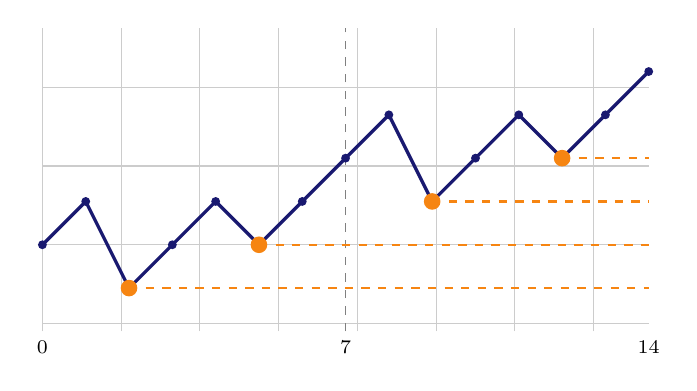
\begin{tikzpicture}[x=0.55cm,y=0.55cm]
\draw[gray!40] (0,-2) grid (14,5);
\draw[gray,dashed] (7,-2) -- (7,5);
\draw[very thick,MidnightBlue] (0,0) -- (1,1) -- (2,-1) -- (3,0) -- (4,1) -- (5,0) -- (6,1) -- (7,2) -- (8,3) -- (9,1) -- (10,2) -- (11,3) -- (12,2) -- (13,3) -- (14,4);
\draw[BurntOrange,thick,dashed] (2,-1) -- (14,-1);
\draw[BurntOrange,thick,dashed] (5,0) -- (14,0);
\draw[BurntOrange,thick,dashed] (9,1) -- (14,1);
\draw[BurntOrange,thick,dashed] (12,2) -- (14,2);
\fill[MidnightBlue] (0,0) circle (1.6pt);
\fill[MidnightBlue] (1,1) circle (1.6pt);
\fill[BurntOrange] (2,-1) circle (3pt);
\fill[MidnightBlue] (3,0) circle (1.6pt);
\fill[MidnightBlue] (4,1) circle (1.6pt);
\fill[BurntOrange] (5,0) circle (3pt);
\fill[MidnightBlue] (6,1) circle (1.6pt);
\fill[MidnightBlue] (7,2) circle (1.6pt);
\fill[MidnightBlue] (8,3) circle (1.6pt);
\fill[BurntOrange] (9,1) circle (3pt);
\fill[MidnightBlue] (10,2) circle (1.6pt);
\fill[MidnightBlue] (11,3) circle (1.6pt);
\fill[BurntOrange] (12,2) circle (3pt);
\fill[MidnightBlue] (13,3) circle (1.6pt);
\fill[MidnightBlue] (14,4) circle (1.6pt);
\node[below,font=\scriptsize] at (0,-2) {$0$};
\node[below,font=\scriptsize] at (7,-2) {$7$};
\node[below,font=\scriptsize] at (14,-2) {$14$};
\end{tikzpicture}
